%!TEX root = New.tex
\section{Background and Motivation}
\label{sec:background}

We are interested in datacenters that are part of a global network of CDN deployments. An individual datacenter is deployed at a location which is close to a region with high demand, and caters mostly to requests from users in that region. 
%A datacenter is provisioned with servers in proportional to the demand in a given region. 
These datacenters are built with commodity servers, each with local storage that is used as for caching content, and commodity switches that are connected in a tree-like topology such that leaf nodes connect to servers, and root nodes providing external connectivity.

%- inter-cache protocol
%- keep two copies for fault tolerance

A load-balancer is a key component of CDN datacenters for ensuring high-quality end-user experience. Load balancer decides which set of servers are going to serve requests for a given content. 
If a server receives a request for a content that is unavailable it its cache, it fetches the content from other servers at the same datacenter or else, from other datacenters. 
By repeatedly sending request for a content to the same set of servers, a load balancer makes it likely that content is available at the server a request is sent to, and therefore the content is immediately returned to the user. Load balancer tries to ensure that traffic at no single server exceeds a given threshold utilization level. The threshold utilization is kept at less than 100\% to tolerate unexpected variations in traffic demand. If any server exceeds this threshold, the load balancer updates its decisions to shift load from the overloaded server to other less loaded servers.

\eat{
---Move this to design
Commonly, datacenter networks use shortest path routing with  ECMP (equal cost multipath) to utilize available path diversity in their topologies. While ECMP has been shown to give sub-optimal results in scenarios where a long-running flow occupies a significant fraction of a link capacity, CDN datacenters can work around the sub-optimality of ECMP due to two reasons. First, most traffic in these datacenters flows in one direction from the servers to the users; each of these flows consumes a small fraction (at most 1\%) of link capacity. Second, these datacenters 
}

Today, entire datacenters are always kept in a powered-on state, and energy savings are limited to hardware-level power management techniques, such as DVFS. But, hardware-level power management is very ineffective both for servers and switches. Servers consume 50-70\% of their peak energy without serving any requests. Networking equipment consumes around 90\% of peak power in idle state. The ineffectiveness of hardware-level power management has led to research on software-level solutions such as consolidation of servers, and energy-minimizing traffic engineering. 

We find two opportunities for enhancing prior work in this area. 

First, we investigate the effect of server shutdown policies on network energy savings. We try to answer two questions: (1) Does reducing the number of active servers help save more network energy? (2) For the same number of active servers, does potential network energy savings depend on which set of servers are kept active? These questions are applicable not only for CDN datacenters, but other datacenters as well. 

Second, we make decision of load balancing, traffic engineering, and content transfers  to ensure that energy savings in CDN datacenters minimally affect user-perceived performance. We guide our design based on answers to following questions: (1) Which set of content should be kept available to ensure that server shutdown policies minimally affect cache hit rates? Specifically, what is the time window, such that if content accessed in the previous time window is kept available despite server shutdown, then cache hit rates are minimally reduced? (2) What is the expected frequency at which load balancing and traffic engineering decisions may need to be updated to avoid overloading servers or network links?

We answer the above questions using examples and based on measurements with content access traces from a large CDN in  Section \ref{sec:jointopt} --- \ref{sec:updatefrequency}.

\subsection{Coordinated server and network shutdown}
\label{sec:jointopt}

\begin{figure}
\centering
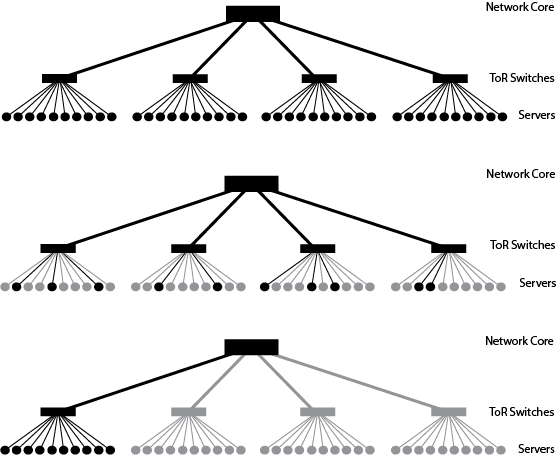
\includegraphics[scale=0.4]{energy/dcTopology.png}
\caption{A datacenter topology. Black components are turned on and grey components are turned off. (Top) All servers and switches are on as is the current practice. (Middle) Demand is consolidated on randomly selected 10 servers and remaining servers are shutoff. All ToR switches must be kept on to provide connectivity to servers. (Bottom) Demand is consolidated on servers in one rack, which allows  servers as well as ToR switches in other racks to be turned off.}
\end{figure}

\subsection{Temporal locality of accesses}
\label{sec:templocality}
2. Because a time window of few hours captures most cache hit rates. Ensuring that content accessed in a recent window is available will ensure most of the benefits.

\subsection{Timescales of operation}
\label{sec:updatefrequency}

Energy minimization are taken at hours timescales to minimize wear and tear due to server shutdown.

Question is how fast should load balancing decisions be taken to ensure a minimal performance impact. We show the  least square errors of difference in content demand on successive time intervals.

%3. How fast should decisions be taken to minimize energy savings and to ensure that performance does not get hurt? 

